\documentclass[journal]{IEEEtran}
% \documentclass[twocolumn,oneside]{IEEEtran/IEEEtran}
% \documentclass[defaultstyle,11pt]{IEEETran}

% \usepackage{showframe}
\usepackage{amssymb}		% to get all AMS symbols
\usepackage{amsthm}
\usepackage{mathtools}
\usepackage{graphicx}		% to insert figures
\usepackage{multirow}
\usepackage{cite}
\usepackage{listings}
\usepackage{booktabs}
\usepackage[percent]{overpic}
\usepackage{subcaption}
\usepackage{xspace}
\usepackage{enumitem}
\usepackage[inkscapelatex=false, inkscapepath=svgsubpath]{svg}
\usepackage{url}
\usepackage[ruled,linesnumbered]{algorithm2e}
\usepackage{placeins}
\usepackage[disable]{todonotes}
 

% Indent paragraphs inside enumerate
\usepackage{enumitem}
\setlist{  
  listparindent=\parindent,
  parsep=0pt,
}
\newcommand{\xyc}{\ensuremath{XY}\xspace}
\newcommand{\xc}{\ensuremath{X}\xspace}
\newcommand{\yc}{\ensuremath{Y}\xspace}
\newcommand{\zc}{\ensuremath{Z}\xspace}

\newcommand{\rzup}{\ensuremath{r_{z,\textrm{up}}}\xspace}
\newcommand{\rzs}{\ensuremath{r_{z,\textrm{s}}}\xspace}

\usepackage{catchfilebetweentags} % for data input
\newcommand{\scanD}[1]{\ExecuteMetaData[cs_data.txt]{#1}}
\newcommand{\baseline}[1]{\ExecuteMetaData[baseline_errors.txt]{#1}}

% *******************************************************************************
% This artificially increases the papersize and margins, so todo notes are legible.
% ***************** WARNING: comment this out for final version. ****************
%\usepackage[paperwidth=734.295pt, textwidth=516pt,
%            marginparsep=5pt, hoffset=10pt, marginparwidth=90pt,
%           textheight=696pt]{geometry}
% Use layouts to display the original dimensions, so we can get as close to that as possible with
% our fake page size.
%\usepackage{layouts}
%textwidth: \printinunitsof{in}\prntlen{\textwidth}
%linewidth: \printinunitsof{in}\prntlen{\linewidth}
% textwidth: \printinunitsof{in}\prntlen{\textheight}

% *******************************************************************************



%%%%%%%%%%%%%%%%%%%%%%%%%%%%%%%%%%%%%%%%%%%%%%%%%%%%%%%%%%%%%%%%%
%%%%%%%%%%%%%%%       BEGIN DOCUMENT...         %%%%%%%%%%%%%%%%%
%%%%%%%%%%%%%%%%%%%%%%%%%%%%%%%%%%%%%%%%%%%%%%%%%%%%%%%%%%%%%%%%%

\begin{document}
\title{Improving the Image Acquisition Rate \\ of an Atomic Force Microscope \\
Through Sub-sampling and Reconstruction}

\author{Roger A. Braker, \textit{Student Member, IEEE}, Yufan Luo, \textit{Student Member, IEEE} , Lucy Y. Pao, \textit{Fellow, IEEE} and Sean B. Andersson, \textit{Senior Member, IEEE, and Member, ASME}
  \thanks{Braker and Pao are with the Dept. of Electrical, Computer, and
    Energy Engineering at the University of Colorado, 425 UCB,
    Boulder, CO 80309, USA. %Phone: +1 (303) 492-2360. Fax:
    +1 (303) 492-2758.}%R. A. Braker (corresponding author
    %roger.braker@colorado.edu) is a graduate student and L.Y. Pao
    %(pao@colorado.edu) is the Palmer  Professor.}
    \thanks{Luo is with the Division of Systems Engineering and Andersson is with the Division of Systems Engineering and the Department of Mechanical Engineering, Boston University, Boston, MA 02215, USA.}
  \thanks{This work was supported in part by the US National Science
    Foundation (NSF Grants CMMI-1234980, CMMI-1234845, CMMI-1562031, and DBI-1352729)  Agilent Technologies,
    Inc., and the Hanse-Wissenschaftskolleg Institute for Advanced Study in Delmenhorst, Germany.} }

\maketitle
\begin{abstract}
  Undersampling-based approaches in Atomic Force Microscopy (AFM) aim
  to reduce the time to acquire an image by reducing the number of
  measurements needed while still maintaining image quality. The approach consists of two components: data acquisition and image reconstruction. While the underlying idea is straightforward, practical implementation of a working scheme involves solving a variety of non-trivial problems. In this
  paper, we describe one such hardware implementation and demonstration based on the use of collections of short scans
  known as $\mu$--paths. Using a commercial AFM, we acquire data on a
  grating sample. Reconstructions are made from these data using
  % three approaches: (1) inpainting, an interpolation technique that
  % diffuses information from sampled locations into unsampled
  % regions, (2)
  % basis-pursuit, a compressive sensing-based algorithm that seeks to
  % minimize a
  % measure of sparsity in the underlying image, and (3)
  a new variant of basis pursuit, Basis Pursuit with Vertical
  Variation, that is designed to reduce artifacts arising from
  the sampling pattern. The quality of the resulting images is
  compared to images from standard raster scans of the same regions at
  comparable imaging rates using both the peak signal-to-noise ratio
  and the structured similarity index metric and a new metric we call
  the relative damage index. These images are compared both to standard raster scans as well as to simple subline sampling where only a subset of the rows of the image are acquired (followed by reconstruction). \textcolor{red}{These experiments demonstrate that at slow scan
  rates, the $\mu-$path scheme produces similar image quality with
  significantly less sampling (and thus less tip-sample interaction)
  and that at high rates, the undersampling scheme produces higher
  quality images than raster scanning.}
\end{abstract}

\section{Introduction}\label{sec:introduction}
% textwidth: \printinunitsof{pt}\prntlen{\textwidth}

% linewidth: \printinunitsof{pt}\prntlen{\linewidth}

% paperwidth: \printinunitsof{pt}\prntlen{\paperwidth}

% marginparwidth: \printinunitsof{pt}\prntlen{\marginparwidth}

% marginsep: \printinunitsof{pt}\prntlen{\marginparsep}

% textheight: \printinunitsof{pt}\prntlen{\textheight}

The Atomic Force Microscope (AFM) is a powerful instrument capable of
imaging sample surface topography, material characteristics, and other
surface properties, with nanometer scale precision. AFMs acquire
information about the sample by monitoring the deflection of the
cantilever caused by the tip-sample interaction force. In general,
% AFMs acquire information about the sample through a variety of
% imaging modes, all of which rely on the deflection of the cantilever
% caused by the tip-sample interaction force. While the details of
% each of the modes are quite different, in general,
feedback control is used to hold the deflection signal constant and
information about the property of interest is inferred from the
applied control or the measured dynamics of the cantilever
\cite{Abramovitch:2007gt}. Because of its versatility, spatial
resolution, and ability to image in vacuum, air, and liquid, AFM is
widely used in a variety of disciplines, including physics, biology,
and materials science
\cite{Dufrene:2017gm,Yang:2017im,Payton:2016hj,Altman:2015ic,Haase:2015eh}.
	
In addition to imaging static samples, AFM is used to study dynamics
in systems with nanometer-scale features
\cite{Yang:2017im,Shibata:2017da,Shibata:2015jd,Ando:2014ja}. The
image acquisition time of conventional AFMs, however, is typically on
the order of seconds to minutes, severely limiting the time-scales
that can be explored. Driven by the need for faster imaging, there
continue to be many active research efforts to overcome this
challenge. Since an AFM is fundamentally a mechanical microscope, many
of the approaches to high-speed AFM (HS-AFM) have focused on
modifications to the physical components. These have included the use
of small, fast cantilevers \cite{Viani:1999tp,
  braunsmann2010high,Adams:2016hg}, the development of faster
actuators \cite{Maroufi:2015gt,Yong:2012kd,Kenton:2012cm}, and
the application of advanced controllers
\cite{Rana:2018es,Yong:2015gr,butterworth2010adaptive,salapaka2002high}.
By combining different techniques, there are current generation,
high-end instruments that can image at rates on the order of 1-10
frames/sec \cite{Ando:2014ja}. However, the fastest rates are achieved
only over small scan ranges and there remain many systems of interest
whose dynamics are faster even than these instruments can achieve. In
addition, there is a large installed base of much slower AFMs that can
benefit from alternative approaches to improving imaging rate.
	
A complimentary class of HS-AFM approaches considers modifications to
the sampling scheme rather than the system mechanics. Alternative scan
trajectories like spirals, cycloids, and Lissajous figures, have been
used in place of the standard raster pattern. While these trajectories are
easier for the actuators to follow, allowing the tip to be moved more
quickly and leading to faster image acquisition on an otherwise
unmodified instrument
\cite{Bazaei:2017dm,Wu:2015dt,Rana:2014bj,Tuma:2012hv,Yong:2010gm}, they are ultimately limited by the vertical bandwidth of
the instrument for regulating the deflection signal \cite{Teo:2016ev}.

A different use of non-raster scan patterns are those that seek to improve imaging rate by reducing sampling rather than increasing speed. This class includes local scanning methods that use the measurements in real-time to steer the tip to focus the scan on features of
interest \cite{Hartman:2018ja,Wen:2018fl,Zhang:2015cf,Huang:2014dw}.
While these have been shown to yield an order of magnitude or better
improvement in imaging rate, they are limited in the class of samples
that can be imaged and do not produce a full image with all the corresponding context.
	
An alternative group of non-raster scanning schemes, introduced in
\cite{song2011video,andersson2012non}, is based on the idea of
undersampling. As with local scanning, data acquisition time is
reduced by reducing the amount of measurements acquired. Unlike local
scanning methods, this approach still presents the full image. Taking
advantage of the redundancy in many natural signals of interest, the
final surface image can be recovered from the limited number of
measured pixels using a variety of different reconstruction methods
such as inpainting or schemes based on the theory of compressive
sensing (CS) \cite{chen2013enhancement,luo2015comparison}. In addition
to the reduced imaging time, undersampling schemes also reduce
tip-sample interactions, thereby reducing the likelihood of tip wear
or sample damage.
	
One simple way to create undersampling schemes is by modifying
existing full scan patterns including raster, spiral, and Lissajous
scanning. For example, subline sampling is generated by randomly
skipping some of the horizontal lines in raster scanning
\cite{han2018reconstruction,chen2013enhancement}. For spiral and
Lissajous patterns, the scan parameters (frequency and amplitude) can
be selected to ensure the trajectory only passes through a desired
fraction of the pixels in the final image. The scanning time for these
smooth undersampling patterns can be estimated based on the proportion
of the pixels in the trajectory. However, results in the literature of
CS make clear that \textit{randomness} in the sampling pattern is
essential for creating good reconstructions in the general case. %The smooth nature of these patterns reduces their randomness and thus leads to less accurate reconstructions than a completely random sampling of the pixels for the same sampling fraction.
	
In AFM, implementing a truly random pattern requires that the tip be
engaged with the surface to collect a measurement, lifted and moved to
the new location, and engaged again.
Because the re-engagement process
is typically slow, this can lead to excessively long image acquisition
times and negate the gains from undersampling \cite{andersson2012non}.
In \cite{maxwell2014compressed}, we introduced an undersampling scheme,
called a $\mu$-path pattern, which consists of short randomly placed,
horizontal scans (illustrated in Fig.~\ref{fig:mu_mask}). It
is designed to balance randomness (to ensure good
reconstruction) with continuous scanning (to reduce the number of tip
engagements).

Our previous work on the $\mu$-path pattern, using theoretical
calculations, simulations, and a preliminary implementation,
demonstrates that the approach can achieve scanning time
reduction while maintaining faithful image reconstruction
\cite{maxwell2014compressed,Luo:2015tu, braker_hardware_2018}. 
The main contributions of this paper relative to that past work are as follows.
\begin{itemize}
\item We introduce a new reconstruction algorithm which is designed to
minimize the artifacts arising from the structure of the $\mu$-path
scanning pattern. This algorithm is described and compared to existing
reconstruction methods through simulations in Sec. \ref{sec:reconstructionMethods}.
\item In our prior experimental prototype \cite{braker_hardware_2018}, we used very basic integral controllers for all three axes for both raster and $\mu$-path scans. Here, we design compensators for each axis using standard loop-shaping techniques (Sec.~\ref{sec:control}), which result in a substantial increase in closed-loop bandwidth (e.g., 50 Hz to 450~Hz for the $Z$-axis).
We show in Sec.~\ref{sec:ff_control} that one of the limitations of $\mu$-path scanning is the discontinuous $X$-axis reference (e.g., in moving between $\mu$-paths) which excites the cross-coupling modes between the $X$ and $Z$ axes, an effect which neither our prior experimental work nor simulation studies accounted for. We mitigate the cross coupling with a feed-forward design.
\item We experimentally compare (Sec. \ref{sec:results}) $\mu$-path scanning to not only full density raster scans but also to coarse raster scans which are interpolated to a full image. This is in contrast to typical sub-line sampling which takes scan lines at random. The clear advantage to a coarse raster scan is that it requires no modification to the instrument, only to the post-processing.
\item The bulk of this work is based on experiment, not simulation, in contrast to prior work by ourselves \cite{luo2015comparison,maxwell2014compressed} and others \cite{han_optimal_2018,jensen_reconstruction_2013,oxvig_structure_2017}. Our main focus here is on delineating the practical issues which must be addressed to effectively realize $\mu$-path scanning, which has only seen limited attention in the past.
\end{itemize}


\begin{figure}
  \centering
  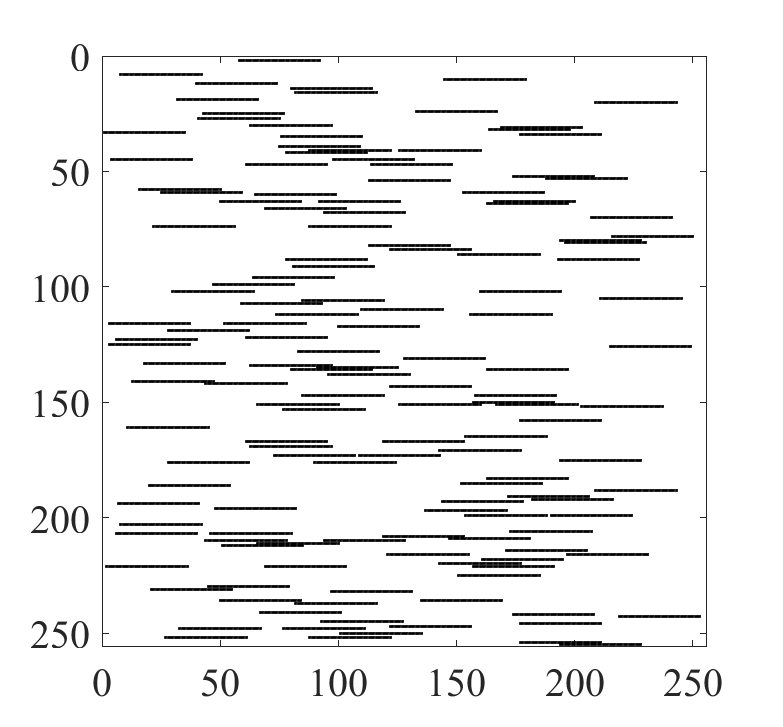
\includegraphics[width=0.65\columnwidth]{figures-SBA/random_mask.pdf}
  \caption{An example of the horizontal $\mu$-path sampling pattern
    for a 256$\times$256 pixel image with 35 pixels in each short scan
    and a total of 20\% pixels scanned.}
  \label{fig:mu_mask}
\end{figure}
% =========================================================================
\section{Reconstruction methods}
\label{sec:reconstructionMethods}
Compressive sensing (CS) is a signal processing technique which aims
at signal reconstruction from a relatively small (sub-Nyquist limit)
number of measurements \cite{carmi2014compressive}. It takes advantage
of the approximate sparsity of real-world signals, that is, that many
coefficients of such signals are close to zero when represented in an
appropriate basis. CS methods seek the true image signal
$x\in\mathbb{R}^n$ from the observation equation,
\begin{equation}\label{op:observation}
  y = R x = RU\eta,
\end{equation}
\noindent where $y\in\mathbb{R}^m$ is the observation vector, $R$ is
an $m\times n$ matrix defining the measurements, $U$ is an $n\times n$
sparsity basis and $\eta$ is the sparse representation of $x$ in the
domain of $U$. In general, $m\ll n$. In an imaging application, where
the underlying signal is a matrix $X\in\mathbb{R}^{h\times s}$, we
take $x=\text{vec}(X)$, where the $\text{vec}(\cdot)$ operator stacks
the columns of a matrix.

\noindent
\begingroup \setlength{\tabcolsep}{1pt}
\begin{figure*}[ht!]
  \centering
  \begin{tabular}{cccccc}
    \textit{\small original image} & \textit{\small BPDN} & \textit{\small BPVV}
    & \textit{\small detail of original} & \textit{\small detail of BPDN} & \textit{\small detail of BPVV} \\
    \includesvg[width=0.16\textwidth]{figures/cs20ng_og.svg}
    %
    & \includesvg[width=0.16\textwidth]{figures/cs20ng_bp.svg}
    %
    & \includesvg[width=0.16\textwidth]{figures/cs20ng_bptv.svg}
    %
    & \includesvg[width=0.16\textwidth]{figures/cs20ng_og_zoom.svg}
    %
    & \includesvg[width=0.16\textwidth]{figures/cs20ng_bp_zoom.svg}
    %
    &   \includesvg[width=0.16\textwidth]{figures/cs20ng_bptv_zoom.svg}\\
    % 
    % ------------------------------
    % Row
    % 2
    % --------------------------------------------
    \includesvg[width=0.16\textwidth]{figures/dna_og.svg}
    %
    & \includesvg[width=0.16\textwidth]{figures/dna_bp.svg}
    %
    & \includesvg[width=0.16\textwidth]{figures/dna_bptv.svg}
    %
    & \includesvg[width=0.16\textwidth]{figures/dna_og_zoom.svg}
    %
    & \includesvg[width=0.16\textwidth]{figures/dna_bp_zoom.svg}
    %
    & \includesvg[width=0.16\textwidth]{figures/dna_bptv_zoom.svg}
  \end{tabular}
  \caption{Reconstruction comparison between BPDN and BPVV. (first
    column) Original raster-scanned image. (second column) BPDN
    reconstruction from random, \textcolor{red}{40 pixel long $\mu$-paths with 25\%
    sampling}. (third column) BPVV reconstruction from the same
    sub-sampled data. (remaining columns) Corresponding details from
    the red boxes indicated in the raster image. The results show that
    BPVV reduces the artifacts arising from the horizontal scans of
    the $\mu$-path pattern that appear in BPDN reconstructions.}
  \label{fig:BPTV_demonstration}
\end{figure*}
\endgroup
	
In the AFM application, the probe can only measure a single pixel at a
time. Thus the rows of $R$ are a subset of those of an $n$ by $n$
identity matrix. Ideally, the sparsity basis and the measurement
matrix $R$ will have a low \textit{mutual coherence}, a measure of how
each of the rows of $R$ (the measurements) ``spreads out'' in the
domain of $U$ \cite{candes2007sparsity}. In the following, we assume
that $U^TU=I$, and in the simulation and experimental results we make the specific choice of $U^T$ as the Discrete Cosine Transform (DCT). The DCT basis
generally keeps a good balance between achieving a low mutual
coherence between $U$ and the $\mu$-path sensing matrices $R$ and
providing a high sparsity for typical AFM sample images.
	
Basis pursuit with denoising (BPDN) is one common realization of the
CS-based reconstruction problem, and is given by the optimization
\begin{equation}
  \min_{x} \left \| U^Tx \right \|_1 \quad
  \text{subj. to}\quad %x\in Q_p = \{x:~\|Rx - y\|_2 < \sigma\} 
  \|Rx-y\|_2 < \sigma \label{op:bp}
\end{equation}
where $\sigma$ represents uncertainty in the measurements. BPDN
essentially searches for the sparsest signal among the candidates
that match the measurements to within the tolerance $\sigma$.

Although BPDN is effective in the general setting, using it for
reconstruction from horizontal $\mu$-path samples often yields
artifacts in the vertical direction (that is, the direction orthogonal
to the $\mu$-path scans) leading to strong discontinuities in the
image. These artifacts grow more prominent as the length of the
$\mu$-paths is increased \cite{maxwell2014compressed}, because these
longer paths lead to increased mutual coherence between the
measurement matrix $R$ and the sparsity basis $U$. However, longer
$\mu$-paths means fewer $\mu$-paths and thus shorter scan times.

To mitigate these affects, we propose a new variant of BPDN that we
term basis pursuit with vertical variation (BPVV). BPVV adds a
vertical total variation penalty in the spatial domain to the
optimization objective. That is, \eqref{op:bp} is modified to \todo{It
  has been my observation that some benefit is gained by including
  $D_h$, but weighting it less than $D_v$. Not sure if we should leave
  it in. If so, BPVV should be BPTV or something.}
\begin{align}
  \min_{x\in Q_p}~f(x) &= \min_{x\in Q_p} \left\|U^Tx\right\|_1
                         + \alpha\left\|D_vx\right\|_1
                         + \beta\left\|D_hx\right\|_1 \label{op:bp_tv}\\
                       &=\min_{x\in Q_p} \left\|W^Tx\right\|_1 \label{op:bp_tvW}
                       % \quad W
                       % = \begin{bmatrix}U&\alpha_hD^T_h&\alpha_vD^T_v \end{bmatrix}^T
                       % \nonumber
\end{align}
where
\begin{equation*}
  W = \begin{bmatrix}U^T&\alpha D_v&\beta D_h \end{bmatrix}
\end{equation*}
with ${D_v x=\text{vec}(\nabla_v X)}$ (resp.,
${D_h x=\text{vec}(\nabla_h X)}$) representing a discrete gradient of
a matrix in the vertical (resp., horizontal) direction (see, e.g.,
\cite[Sec. 6.1,]{becker_nesta_2011}). 
% and
% \begin{align*}
%   (\nabla_v X)_{i,j} = 
%   \begin{cases}
%     X_{i+1,j} - X_{i,j}, & 1\leq i<h,~ 1\leq j\leq s,\\
%     0, & \phantom{:}i=h,~\phantom{:::::} 1\leq j\leq s.
%   \end{cases}\\
%   (\nabla_h X)_{i,j} =
%   \begin{cases}
%     X_{i,j+1} - X_{i,j}, & 1\leq i\leq h,~1\leq j<s \\
%     0, & \phantom{}1\leq i\leq,~\phantom{:::} j=s
%   \end{cases}
% \end{align*}
Thus, in \eqref{op:bp_tv}, $\left \| D_v x \right \|_1$ (resp.,
$\left \| D_h x \right \|_1$) is the total variation (TV) of the
signal in the vertical (resp., horizontal) direction. The parameters
$\alpha$ and $\beta$ are weighting parameters. The description of BPVV
in \eqref{op:bp_tvW} can be interpreted as changing our assumption of
sparsity in the DCT basis to assuming sparsity in an overcomplete
dictionary \cite{candes_redundant_2011}. \todo{I believe this is
  correct: Sean/Yufan can you confirm or reject?} When written as
\eqref{op:bp_tvW}, the problem is in a form that may be solved with
NESTA~\cite{becker_nesta_2011}. Note that the BPVV designation technically holds only for $\beta=0$; our experience, however, shows that including a small but nonzero $\beta$ (relative to $\alpha$) improves reconstruction.

% For completeness, we give an overview here. To that end, we re-write
% the cost $f(x)$ in \eqref{op:bp_tvW} as
% \begin{equation*}
%   f(x) = \max_{u\in Q_d} \left\langle u, W^Tx \right\rangle,\quad Q_d = \{u:~||u||_{\infty} \leq 1\}.
% \end{equation*}

% One of the core features of the NESTA algorithm is to replace the
% non-smooth functional $f(x)$ with a smoothed approximation
% \begin{equation}
%   f_{\mu} = \max_{u\in Q_d} \left\langle u,
%     W^T x \right\rangle - \frac{\mu}{2}||u||_2^2. \label{eqn:fcn_prox}
% \end{equation}
% The gradient of \eqref{eqn:fcn_prox} is given by
% \begin{equation*}
%   \nabla f_{\mu}(x)[i] = Wu_{\mu}(x)
% \end{equation*}
% where
% \begin{equation*}
%   (u_{\mu}(x))[i] = 
% \begin{cases}
%   \mu^{-1}(W^Tx)[i], & |W^T x[i]| < \mu,\\
%   \text{sgn}(W^T x[i]), & \text{else}.
% \end{cases}
% \end{equation*}
% The optimization \eqref{op:bp_tv} may now be solved using
% Algorithm~\ref{ag:NESTA}.

% \begin{algorithm}
%   \SetKwInOut{Initialize}{Initialize} \SetKwInOut{Output}{Output}
		
%   \Initialize{$x \in Q_p, \mu=0.9||W^T x_0||_{\infty}$,
%   $L_{\mu} = \frac{1}{\mu}||W||^2_2$}
%     %   $x^{k+1} = x^{k}$\\
%   \While{$\mu < \mu_{\textrm{final}}$ } {
%   $k=0$\\
%   \While{$\Delta f_{\mu} > \delta$} {
%   $\alpha_k = \frac{1}{2}(k+1)$ \\
%   $\tau_k = \frac{2}{k+3}$ \\
%   $\displaystyle y_k = \text{arg } \min_{x\in Q_p}
%   \frac{L_{\mu}}{2}||x - x_k||_2^2 + \langle \nabla f(x_k),~ x\rangle$\\
%   $\displaystyle {z_k = \text{arg } \min_{x\in Q_p}
%   \frac{L_{\mu}}{2}||x-x_0||_2^2 +
%   \langle \sum_{i=0}^k \alpha_i \nabla f(x_i), ~x \rangle}$\\
%   $x_{k+1} = \tau_kz_k + (1-\tau_k)y_k$\\
%   $k \leftarrow k + 1$\\
% }
%   $x_0 = x_k$\\
%   $\mu = \gamma \mu$\\
%   $L_{\mu} = (1/\mu)||W||^2_2$ } \Output{Reconstruction $x_k$}
%   \caption{NESTA algorithm}
%   \label{ag:NESTA}
% \end{algorithm}
% \todo{seems like a waste of space to reprint the algo, since its
% really no different than the reference}


% In the termination condition for the inner loop,
% $\Delta f_{\mu} = |f_{\mu}(x_k) -
% \bar{f}_{\mu}(x_k)|/\bar{f}_{\mu}(x_k)$ where
% \begin{equation}
% \bar{f}_{\mu}(x_k) = \frac{1}{\min\{10, k\}} \sum_{\ell=1}^{\min\{10,k\}} f_{\mu}(x_{k-\ell})
% \end{equation}
% When $RR^T=I$, the sub-problems in lines 6 and 7 have a closed-form
% solution. Details can be found in~\cite{becker_nesta_2011}.

% % The sub-problems in lines 6 and 7 have the form
% % \begin{equation}
% %   p = \textrm{arg } \min_{x\in Q_p} \frac{L}{2}||x - r|| + \langle
% %   g,~x - r\rangle
% % \end{equation}
% % for some vectors $g$ and $r$ and, as shown
% % in~\cite{becker_nesta_2011}, have a closed-form solution given by
% % \begin{align}
% %   \lambda & = \textrm{max}(0, \sigma^{-1}\left| b -
% %     Rq\right| - L\\
% %   q &= r - L^{-1}g\\
% %   p &= \left(I - \frac{\lambda}{\lambda + L}
% %     R^TR\right)\left( \frac{\lambda}{L}R^Tb + q\right).
% % \end{align}


A simulation comparison between BPDN and BPVV is shown in
Fig.~\ref{fig:BPTV_demonstration}. The first column shows two raster
scans: the top is a 512 by 512 pixel image of a CS-20NG grating (Ted Pella, USA) acquired
with an Agilent 5400 AFM and the bottom is a 256 by 256 pixel image of
DNA acquired with an Agilent 5500 AFM. For the CS-20NG grating, we
sampled 15\% of the pixels with 50 pixel $\mu$-paths and 25\%
of the DNA image with 25 pixel long $\mu$-paths. The second columns
shows the full frame reconstructions using BPDN and the third columns
shows the result using BPVV (\textcolor{red}{with $\alpha = ??$ and $\beta = ??$}). The fourth column zooms in on the region
indicated by the red box in column one. Similarly, the fifth and six
columns show the detail of the reconstructions. The reconstruction
results show the artifacts apparent in the BPDN reconstruction are
largely mitigated using BPVV. Thus, in the remainder of the paper, we
focus exclusively on BPVV. These reconstructions wth BPVV took about
1.5 seconds for the DNA image and about 7 seconds for the
CS-20NG (on a typical laptop computer).
	

% =========================================================================
\section{Experimental setup} \label{sec:experimentalSetup}
% =========================================================================
\begin{figure}[ht!]
  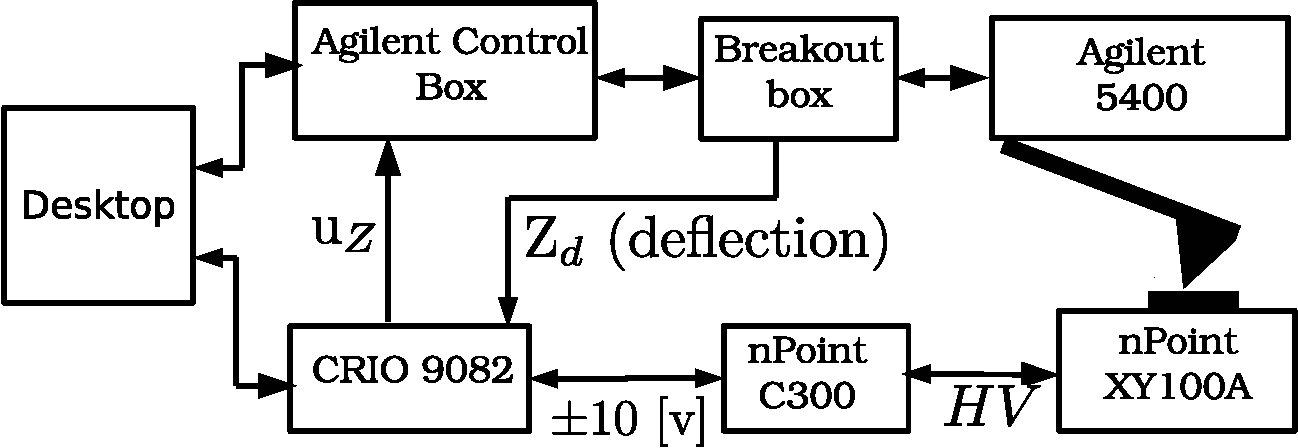
\includegraphics[width=1\columnwidth]{figures/exp_setup.pdf}
  \caption{Schematic diagram of the expermental AFM setup.}
  \label{fig:exp_setup}
\end{figure}

Our experimental setup, illustrated in Fig.~\ref{fig:exp_setup},
consists of an Agilent 5400 AFM retrofitted with an nPoint NPXY100A
piezoelectric stage, a cRIO-9082 embedded controller (National
Instruments), and a standard desktop computer.

Through a breakout box, the Agilent 5400 provides access to the
$Z$-axis deflection signal. When the Agilent software is set to
open-loop mode, a $\pm10$~volt input on the standard control box
allows control of the $Z$-axis of the N9524a piezo scanner, which has
a total range of 7 $\mu$m. Initial (coarse) engagement of the tip to
the sample is performed using the PicoView software before control is
handed over to the custom controllers.
	
All control logic is programmed using LabVIEW 2019 and compiled to a
Xilinx Spartan-6 LX150 Field Programmable Gate Array (FPGA) inside the
cRIO-9082. The cRIO includes 16-bit, 100 kHz analog-to-digital input (NI-9215)) and digital-to-analog output (NI-9263) modules.
%a 16-Bit, 100 kHz NI-9215analog-to-digital input module and a 16-Bit, 100 kHz NI-9263 digital-to-analog output module. 
All control loops are implemented
using a 25 kHz sampling rate.


% =========================================================================
\section{Implementation}\label{sec:implementation}
% =========================================================================

Implementing the $\mu$-path scheme involves operating the AFM in
several distinct stages. In the $XY$-direction, the system transitions
from tracking a step command in the transition to a new measurement
location to tracking a short ramp during the actual $\mu$-path scan.
In the $Z$-direction, the system must transition between tip descent,
surface scanning, and tip retraction. Two cycles of this sequential
process are illustrated by the time series in Fig.~\ref{fig:cs_cycle}.
The following subsections describe in more detail several features of
the CS scanning process.

Transition between, and operation in, these different stages is
implemented as a simple state machine, summarized in
Table~\ref{tab:cs_tasks}. The main job of the state machine is to
adjust the reference signals to accomplish each task. In the
following, $r_X$ and $r_Y$ refer to the references for the
$X$ and $Y$ axes while $r_{Z,s}$ and $\rzup$ refer to the $Z$-axis
setpoints during scanning and retraction, respectively.

\begin{table}[h!]
  \centering
  \caption{Summary of the tasks for $\mu$-path scanning.}
  \begin{tabular}{lccc}
    state & $r_X$,$r_Y$ & $r_Z$ & next-state\\
    \toprule
    (1) $XY$-move & setpoint & $r_Z = \rzup$ & (2)\\
    (2) tip-engage & setpoint & $r_Z = \rzs$ & (3)\\
    (3) pre-scan & ramp & $r_Z = \rzs$ & (4)\\
    (4) $\mu$-path scan & ramp & $r_Z = \rzs$ & (5)\\
    (5) tip up & setpoint & $r_Z = \rzup$ & (1)\\
  \end{tabular}
  \label{tab:cs_tasks}
\end{table}

  
\subsection{Cantilever does not need to fully disengage.}
\todo{Not clear to me yet that friction is useful if I scan parallel
  to cantilever. Also not clear to me that the normal force and shear
  force are orthogonal concepts. Maybe the macroscopic analogy breaks
  down, but thinking of a knife pushed into a surface and then
  dragged...} 
  
In order to minimize the scanning time, tip tip should be moved as fast as possible when trainsitioning between $\mu$-path locations (state (1)). Since such speeds can be beyond the bandwidth of the $z-$axis controller, it is important to reduce the tip-sample interaction force to prevent tip sear and sample damage. In our initial implementation, this was achieved by 
%In our initial implementation
\cite{braker_hardware_2018}, we insisted that the during
tip-retraction (state (5)), the cantilever tip should fully break
contact with the surface. Here, we impose no such requirement. Rather,
we change the $Z$-setpoint during tip-retraction to only pull away far
enough that the deflection signal stays low (i.e., below the scanning
setpoint), even while we run across the surface. We choose \rzup so
that the interaction between the tip and sample becomes purely
adhesive. In general, stable imaging is not possible at \rzup and
complete dis-engagement occasionally occurs. This can be seen in bottom pane of
Fig.~\ref{fig:cs_cycle} during the second $XY$-move (black portion) where the tip detaches partway through the move.
%Fig.~\ref{fig:afm_bd_dinv} which selects either the scanning setpoint $r_{Z,s}$ or the retraction setpoint $r_{Z,\textrm{up}}$ based the current state.
When dis-engagement does occur, the $Z$-axis control loop implements an anti-windup scheme to prevent the control from saturating.


Only moving the tip into the adhesive region during the $XY$ move saves considerable time
compared to completely detaching the tip between each $\mu$-path. By eliminating the normal force into the sample, we are able to take dozens of images with a single probe without a noticeable degradation in image quality. However, completely characterizing the damage done to the tip and sample with this scheme compared complete detachment (which can also damage the probe \cite{meyer_atomic_1992}), remains an outstanding goal.

\begin{figure}[t!]
  \centering \includesvg[width=1\columnwidth]{figures/cs_cycle.svg}
  \caption{Several CS cycles. Each state is indicated by color.}
  \label{fig:cs_cycle}
\end{figure}

\begin{figure*}[ht!]
  \centering
  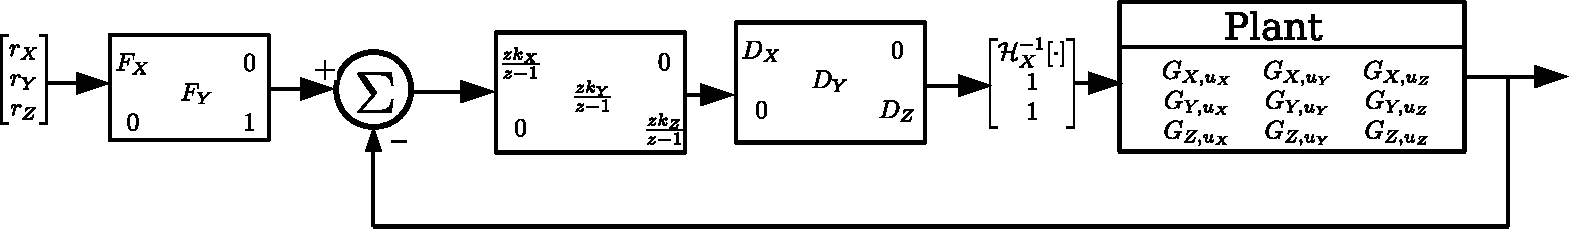
\includegraphics[width=1\textwidth]{figures/AFM_loop_xyz.pdf}
  \caption{Block diagram of the AFM control loop for all three axes.
    Not shown is anti-windup for the $Z$-axis integrator, which is active
    when $r_Z=\rzup$ (states 1 and 5) where sensor saturation is possible.}
  \label{fig:afm_bd_dinv}
\end{figure*}
\subsection{The pre-scan}
After the tip-descent, we begin scanning in a ``pre-scan'' phase
(state (3)), which is the turquoise ``tip settle'' portion of the trajectories in
Fig.~\ref{fig:cs_cycle}. There are two reasons for this. First, we
have observed that there is less noise in the deflection signal while
the $XY$-stage is in motion compared to sitting still. More
importantly, it lets us bring the $X$-axis to its scanning velocity at
the same time the transients from the $Z$-axis die out. Without this,
we must extend the $\mu$-path by a distance equal to the steady-state
error following a ramp. For an arbitrary scan speed, this means the
$\mu$-path scan would need an extra
\begin{equation}
  N = \left\lceil\lim_{z\rightarrow 1} \frac{1-H_x}{z-1}\right\rceil
\end{equation}
time steps, where $H_x$ is closed-loop transfer function for the
$x$-axis. For our system $N=111$. By initiating the scan while the
$Z$-axis settles, we eliminate much of this overhead.

\subsection{Control}\label{sec:control}
% \begin{figure}
%   \centering
%   \includesvg[width=1\columnwidth]{figures/z_control_design.svg}
%   \caption{FRFs of the $Z$-axis. The blue curve is the open loop
%   response from $u_Z$ to deflection. By inverting the bending mode
%   at 215~Hz, we achieve the black curve in closed-loop.}
%   \label{fig:z_control}
% \end{figure}
The control structure for each axis, shown in the block diagram in
Fig.~\ref{fig:afm_bd_dinv}, is similar and essentially consists of a
set of filters in series with a PI controller. The open-loop frequency
responses for the $X$ and $Y$ axes are shown as the black curves in
Fig.~\ref{fig:mimo_frf_uxuy} and for the $Z$-axis in
Fig.~\ref{fig:z_control}. The first resonance of each axis is the
bending mode, which appears at 215~Hz for the $Z$ axis and about
350~Hz for the $X$ and $Y$ axes.

The filter portion of the $Z$-axis controller $D_Z$ is second-order
and simply inverts the complex-conjugate pole-zero pair at 215~Hz.
This allows the gain of the PI controller to be increased
substantially. The closed-loop achieves a bandwidth of about 450~Hz,
as shown by the red curve in Fig.~\ref{fig:z_control}. Without this
inversion, the bandwidth is limited to about 50~Hz.

We take a similar approach for the $X$ and $Y$ axes. The filters $D_X$
and $D_Y$ invert the bending modes at 350~Hz and add notch filters at
the main resonant peaks near 650~Hz. The resulting closed-loop
transfer functions are shown as the red curves in
Fig.~\ref{fig:mimo_frf_uxuy}.

In general, the $X$-axis positioning requirements are more stringent
for both CS and raster scanning. Due to the step inputs the $X$-axis
must track, we have found that compensating hysteresis and creep to be
particular helpful during $\mu$-path scanning. Thus, the $X$-axis
compensator also includes an inverse creep and hysteresis model. The
hysteresis model is a modified Prandtl-Ishlinskii type model and is
based on the work of \cite{kuhnen_modeling_2003}, while the drift
compensation models the piezo creep as a simple second-order transfer
function with real poles and zeros. In Fig.~\ref{fig:afm_bd_dinv}, the
hysteresis inversion is indicated by $\mathcal{H}^{-1}[\cdot]$. We
have found that the inclusion of these extra compensators limits the
overshoot of the $X$-axis during larger moves between different
$\mu$-paths (e.g., without them, the $X$-axis trajectory in
Fig.~\ref{fig:with_ff} would show noticeable overshoot). More details
on fitting the creep and hysteresis models can be found in our other
work \cite{braker_afmmpc_2019}.

\begin{figure*}
  \centering
  \begin{subfigure}[b]{.65\textwidth}
    \includesvg[width=1\textwidth]{figures/MIMO_CL_uxuy.svg}
    \caption{}\label{fig:mimo_frf_uxuy}
  \end{subfigure}\hfill
  \begin{subfigure}[b]{.34\textwidth}
    \includesvg[width=1\textwidth]{figures/with_wo_ff.svg}
    \caption{}\label{fig:with_ff}
    \vspace{2ex}
    \includesvg[width=1\textwidth]{figures/z_control_design.svg}
    \caption{}\label{fig:z_control}
  \end{subfigure}
  \caption{(a) MIMO closed and open-loop frequency-response functions (FRFs), showing the dramatic
    affect on $G_{Z,u_X}$ and $G_{Z,u_Y}$ when the feedforward
    compensators are used for the $X$ and $Y$ axes. (b) The vertical
    control $u_Z$ (top) after a large move in the $X$-direction
    (bottom) without (left column) and with (right column) the
    feedforward compensation. (c) Frequency response of the $Z$-axis
    in open-loop (black) and closed-loop (red). }
\end{figure*}


% We note that the $z$-axis control described here operates the AFM in
% constant force mode during imaging. It is straightforward to perform
% scanning under different AFM modes, such as tapping mode, simply by
% adjusting the signals and control involved in the vertical loop.

\subsection{Feedforward Control}\label{sec:ff_control}
Unfortunately, as the bottom row of plots in
Fig.~\ref{fig:mimo_frf_uxuy} makes clear, there is a strong
cross-coupling from the horizontal plane to the $Z$ axis (the coupling
from $u_Z$ to the $X$ and $Y$ axes is very weak, and so is not shown).
Our SISO control scheme does little to attenuate the resonances of
$G_{Z,u_X}$ and $G_{Z,u_Y}$. In particular, there are modes in both
these transfer functions at 215 and 505 Hz that do not appear in a
SISO model of $G_{X,u_X}$ or $G_{Y,u_Y}$.

For raster scans, the frequency content of the $X$-axis reference
(which is a triangle wave) decays like $1/n^2$ with a gain
proportional to the raster frequency. In contrast, the $X$-axis
reference for a $\mu$-path scan is composed of a sequence of steps and
ramps. The inclusion of the (discontinuous) steps means we should
expect the $\mu$-path $X$ reference to decay like $1/n$. Thus, while
the cross-coupling can induce $Z$-axis vibrations for faster raster
scans, it is especially problematic for $\mu$-path scanning. This is
illustrated in the left column of Fig.~\ref{fig:with_ff}, which shows
a CS cycle during which the $X$-axis makes a 5 micron move, which
induces excessively large vibrations in the vertical control.

In principle, one could mitigate these issues with a full MIMO control
design. In this work, we opt for a much simpler feedforward scheme.
For CS scanning, we insert feed-forward filters ($F_X$ and $F_Y$ in
Fig.~\ref{fig:afm_bd_dinv}) with three notches: at 215~Hz, 350~Hz, and 505~Hz. Both filters are shown in Fig.~\ref{fig:mimo_frf_uxuy} as the dashed-pink curves and the
resulting overall FRF is shown as the blue curves, which show a
dramatic reduction in the cross coupling. A similar effect could be
achieve by using a simple low-pass filter. However, to achieve the
same 40~dB of attenuation of the mode at 215~Hz, would require, e.g.,
that a two-pole low-pass filter have its cut-off frequency at about
20~Hz. Thus, while our feedforward scheme slows the $X$-axis down, we
achieve better bandwidth than we would with a simple low-pass filter.

For raster scanning, we set $F_X=F_Y=1$ and instead take advantage of
the periodicity of the $X$-axis reference, which is a triangle wave.
We modify the triangle wave to a truncated Fourier series, where each
Fourier coefficient is scaled by the inverse of the closed-loop FRF at
the corresponding frequency. See, e.g., \cite{clayton_review_2009} for
more details on this strategy. We truncate this series such that the
highest frequency is smaller than 200 Hz, which means that we should
never excite the problematic $G_{Z,u_X}$ modes. This scheme implies
that the effective bandwidth of the $X$-axis controller is higher
while raster scanning than while CS-scanning. On the other hand, it
also implies that for faster scan rates, fewer Fourier
coefficients are used, and so the approximation to a triangle wave is
worse.

\section{Metrics}\label{sec:rdi}
In section~\ref{sec:results} we use three metrics to assess our
results. The first two seek to quantify image quality between two images.
Define a master image as $X$ and a reconstruction or corrupted version
as $Y$, with each having $s\times h=m$ pixels. Let $x=\textrm{vec}(X)$
and $y=\textrm{vec}(Y)$. Let $L$ be the dynamic range of the master
image $x$. Then the peak signal to noise ratio (PSNR) is given by
\begin{equation*}
  \text{PSNR}(x,y) = 10\log_{10}\frac{L^2}
  {\sqrt{\frac{1}{m} \sum_{i=1}^{m}( x_{i} - y_{i})^2 }}.
\end{equation*}

The goal of the SSIM is to compare two image's structure,
luminescence, and contrast and is built up from the means ($\mu_x$ and
$\mu_y$), standard deviations ($\sigma_x$ and $\sigma_y$), and
covariance ($\sigma_{xy}$) of the image vectors $x$ and $y$. The SSIM definition used in this paper is
\begin{equation*}
  \text{SSIM}(x,y) = \frac{(2\mu_x\mu_y + C_1)(2\sigma_{xy}+C_2)}
  {(\mu_x^2 + \mu_y^2 + C_1)(\sigma_x^2 + \sigma_y^2 + C_2)}
\end{equation*}
where the constants $C_1$ and $C_2$ are regularizing constants to
prevent singularity if, e.g., $\mu_x=\mu_y=0$. We use the default
values suggested in \cite{wang_image_2004} of $C_1=(0.01L)^2$ and
${C_2=(0.03L)^2}$, where again, $L$ is the dynamic range. In general
two images which are identical will yield an infinite PSNR and an SSIM
of 1.

\subsection{Limitations of SSIM and PSNR}\label{sec:limits}
The SSIM and PSNR have become reasonably popular in studies comparing
simulated AFM image reconstructions \cite{oxvig_structure_2017,
  han_optimal_2018, Luo_nano_2015}. However, it remains somewhat of an
open question how to best compare experimental AFM images. While we
use the SSIM and PSNR in Sec.~\ref{sec:results}, we believe those
numbers should be interpreted with some caution. In our experimental
setup, actuation in the $XY$-plane happens via the nPoint piezo stage
and the $XY$-direction of the original piezo scanner is uncontrolled.
This leads to substantial drift between images. To illustrate this, we
took a sequence of 6 raster scans of a sample grating, each at a 1~Hz
scan rate over a 5 micron by 5 micron area. The left image of
Fig.~\ref{fig:baseline_errors} shows the error between the first and
sixth image. The PSNR and SSIM between the first and second images are
\baseline{one2twoNoAlgnPsnr} and \baseline{one2twoNoAlgnSsim}; between
the first and sixth are \baseline{one2sixNoAlgnPsnr} and
\baseline{one2sixNoAlgnSsim}, respectively, even though on their own
each image appears to have good quality.

To mitigate this affect, we use an image alignment technique based on
the 2D cross-correlation between each image. Essentially, this takes a
sub-slice of the master (first) image (here, a 25 pixel inset on each
edge), and finds the offset in the other image that produces the
smallest error. The result of this procedure is shown in the right
image of Fig.~\ref{fig:baseline_errors}. Although the situation is
improved compared to the un-aligned images, there is still noticeable
stretching (the upper and lower portions appear considerably worse
than the middle). Notably however, with the alignment technique, the
SSIM is \baseline{one2twoAlgnSsim} for both the second and sixth image
images and the PSNR increases to \baseline{one2twoAlgnPsnr} and
\baseline{one2sixAlgnPsnr} respectively.

\begin{figure}[t!]
  \centering
  % \includesvg[width=0.7\columnwidth]{figures/baseline_errors_aligned_1Hz.svg}
  \includesvg[width=0.7\columnwidth]{figures/baseline_errors_1and6.svg}
  \caption{Errors between the first and sixth raster scans in a
    sequence of six 1.0~Hz raster scans. (left) Errors without
    alignment (right) The same data but aligned via cross
    correlation.}
  \label{fig:baseline_errors}
\end{figure}


\subsection{A new metric}
The PSNR and SSIM metrics only assess the similarity of two images.
However, in AFM imaging, pure image quality is not the only concern,
particularly for delicate samples. What is needed is a figure of merit
for how much damage was done to a specimen during the imaging process.
While damage to the specimen is not really a concern while imaging a
hard calibration grating, it plays a prominent role for biological
samples~\cite{ando_highspeed_2008}, though damage to the probe itself
is still a concern. In general, the faster the scan rate, the more
difficulty the $Z$-axis control will have in following the sample
surface, which results in a larger $Z_d$ over more time. The actual
damage done by a given $Z_d$ will depend on the spring constant of the
cantilever and the softness of the specimen. Nonetheless, we propose a
metric, which we call the Relative Damage Index (RDI) which computes
the power in the deflection signal for a given scan. That is,

\begin{align}
  \text{RDI} &= \frac{1}{T_s}\sum_{k=0}^N \frac{1}{k} \left(Z_{d,k} - r_{Z,s}\right)^2 \label{eqn:RDI}\\
\end{align}
The idea behind the RDI is that increased scan rates lead to larger
deflection signals (and thereby increased force into the specimen) at
each surface feature, which the RDI accumulates.

\section{Experimental Results}\label{sec:results}
We compared $\mu$-path scanning to two scenarios. First, we compare it
to full resolution raster scans at several scan rates in
Sec.~\ref{sec:cp_full}. Second, we compare to coarse raster scans in
Sec.~\ref{sec:cp_subline}.

\subsection{Comparison to full raster}\label{sec:cp_full}
We took scans of a Ted Pella CS-20NG sample grating over an area with
holes on a 500 nm pitch. The holes are 20 nm deep. We scanned 5 micron
by 5 micron images using standard raster scans with 512 lines. For the
raster scans, we took scans at 1.0~Hz, 2.5~Hz, 5.0~Hz, 8.0~Hz and
10~Hz. We also took $\mu$-path scans with densities at 12.5\% and
25\% and reconstructed 512 by 512 pixel images. The CS scans were
taken with scan velocities equivalent to raster scan rates of 1.0~Hz,
2.0~Hz, 4.0~Hz, 5.0~Hz and 8.0~Hz. For all CS scans, the $\mu$-paths are
$\scanD{muLenNM}$ nm long, which translates to $\scanD{muLenPix}$
pixels.

The free value of the deflection signal was approximately $-0.6$ volts
and we set the scanning reference to ${\rzs=\scanD{spScan}}$~volts
(for both raster and CS) and the withdraw reference to
${\rzup=\scanD{spMv}}$ volts. We set the $XY$-settle boundary to
$\pm \scanD{xyBoundaryMic}$ microns and required $\scanD{xySetSamps}$
samples within this boundary before moving to the $Z$-engage state.
The pre-scan length was $\scanD{preScanSamples}$ time steps. The
cantilever was a Budget Sensors ContAI-G, with a nominal length of 450
microns and spring constant of $0.2$~N/m.

% \SSData{G2}$& $g_6 = \SSData{G6}
The CS scans were reconstructed with BPVV. We set
${\alpha=\scanD{alph}}$ and ${\beta=\scanD{alpv}}$. For the
raster scans, we discard data from the re-trace and divided the
remaining data for each scan line into 512 bins based on the \xc
sensor measurements. We then average the data in each bin to obtain
the value of one pixel. To remove the affects of piezo creep and
sample tilt, we then de-trend each individual line. De-trending each
line causes the flat portion between the holes in the horizontal
direction to appear at a different height than the flat portion
between holes in the vertical direction. To remove this effect, we
select a column of pixels on the left and right side of each image
that does not cross any holes (i.e., a vertical line through the flat
area), and register each scan line to a common height along these columns.
This step eases comparison with the CS scans and was inspired by a
feature in the AFM image processing toolbox \texttt{SPIW} \cite{spiw}.
The resulting images are shown in Fig.~\ref{fig:resultsF1_images}. The
color maps represent a range of $\pm$20 nm. The rows of pixels
indicated by the red lines are shown as cross sections
Fig.~\ref{fig:pixel_rows}.

\begin{figure*}
  \centering
  \includesvg[scale=.98]{figures/cs_raster_images_6-5-2019.svg}
  \caption{Raster and compressed sensing images of a 5 micron square
    area of the CS-20NG grating. All images are 512$\times$512 pixels:
    the raster images marked as 64 and 128 lines have been
    interpolated. The rows of pixels indicated by the red line are
    shown in Fig.~\ref{fig:pixel_rows}.}
  \label{fig:resultsF1_images}
\end{figure*}

% \begin{table}[t!]
%   \centering
%   \caption{Performance metrics for raster and CS scans.}
%   \begin{tabular}{cccccc}
%     \input{tables/cs_raster_table_6-5-2019_muInf_dct2.tex}
%   \end{tabular}
%   \label{tab:rast_vs_cs_v1}
% \end{table}

\begin{table}[t!]
  \centering
  \caption{Breakdown of state times for the CS scans shown in
    Fig.~\ref{fig:resultsF1_images}. All times are in seconds.}
  \label{tab:final_state_times}
  \begin{tabular}{ccccccc}
    description & move & engage & pre-scan & scan & tip-up & total\\
\toprule
1.0 Hz, 12.4~\% &6.16 & 1.13 & 3.82 & 32.25 & 0.24 & 43.60\\
5.0 Hz, 12.4~\% &6.09 & 1.01 & 3.82 & 6.73 & 0.08 & 17.73\\
8.0 Hz, 12.7~\% &6.14 & 1.02 & 3.82 & 4.35 & 0.08 & 15.40\\
1.0 Hz, 24.0~\% &11.84 & 2.40 & 7.62 & 64.41 & 0.15 & 86.42\\
5.0 Hz, 25.3~\% &11.54 & 2.19 & 7.62 & 13.44 & 0.53 & 35.32\\
8.0 Hz, 24.8~\% &11.73 & 2.06 & 7.62 & 8.68 & 0.15 & 30.25\\

  \end{tabular}
\end{table}

\begin{figure}
  \includesvg[width=1\columnwidth]{figures/cs_raster_pixel_rows_6-5-2019.svg}
  \caption{Rows of pixels, as indicated by the red lines in
    Fig.~\ref{fig:resultsF1_images}. For clarity, not all images are
    included.}
  \label{fig:pixel_rows}
\end{figure}
For each raster scan and each CS scan, we computed the SSIM and PSNR
using the 1~Hz raster scan as the master and also computed the RDI
metric. These are plotted against total acquisition time in
Fig.~\ref{fig:time_vs_metrics}. Unfortunately, the
SSIM and PSNR metrics are not particularly illuminating. There are
several inconsistencies. For example, it makes no sense that the 1~Hz CS
scan at 25\% has a \emph{worse} PSNR and SSIM than the 5~Hz scan; nor
does it make sense that the 8~Hz full raster scan has a worse SSIM and
PSNR than the 10~Hz full raster scan.

\begin{figure*}[t!]
  \centering
  \begin{subfigure}{0.329\linewidth}
    \centering
    \includesvg[width=1\columnwidth]{figures/cs_rast_time_vs_ssim.svg}
    \caption{}
    \label{fig:time_ssim}
  \end{subfigure}
  \begin{subfigure}{0.329\linewidth}
    \centering
    \includesvg[width=1\columnwidth]{figures/cs_rast_time_vs_psnr.svg}
    \caption{}
    \label{fig:time_psnr}
  \end{subfigure}
  \begin{subfigure}{0.329\linewidth}
    \centering
    \includesvg[width=1\columnwidth]{figures/cs_rast_damage.svg}
    \caption{}
    \label{fig:time_damage}
  \end{subfigure}
  \caption{Metrics for raster scan at 512, 128 and 64 lines and
    $\mu$-path scans at 12.5\% and 25\% sampling. The scan rate is
    indicated by color while the scan style is indicated by marker
    style. (a) SSIM as a function of total acquisition time. (b) PSNR
    as a function of total acquisition time. (c) RDI as a function of
    total acquisition time.}
  \label{fig:time_vs_metrics}
\end{figure*}


Things are clearer if we plot the RDI for each scan against total
acquisition time, which is shown in Fig.~\ref{fig:time_damage}, and
this is where CS seems to shine. As one would expect, as imaging time
decreases, the RDI for each scan type increases. From
Fig.~\ref{fig:time_damage}, we see that for a fixed RDI, CS has a
faster imaging acquisition rate. The amount of improvement is best if
we need a very low RDI: for example, if we want to hold the RDI below~2, then we have to take the 1~Hz raster scan (512 seconds) while we
can achieve the same RDI via CS in about 42 seconds with the 12.5\%
sampling, which is a speed improvement of over a factor of 10. The higher of an
RDI we are willing to tolerate, the advantage of CS over raster
narrows. For example, the 8~Hz raster scan and 8~Hz, 12.5\% CS scan
have comparable RDIs, but now CS is only about 5 times faster. This is
a result of the constant overhead imposed by the engage/disengage and
$XY$-move states in CS which remains constant for different scan
rates.

\subsection{Comparison to Sub-line Sampling} \label{sec:cp_subline}
Many sub-line sampling papers assume that the lines to sample are
selected randomly \cite{han_optimal_2018, Luo_nano_2015}. An even
simpler alternative to $\mu$-path sampling is to simply take a
standard raster scan with fewer lines. This is the technique we
consider in this subsection, by scanning images with 128 and 64 lines.
For each of these scenarios, we first divide the data for each line
into 512 bins. This gives an image that is 128 (resp., 64) pixels by
512 pixels. We then linearly interpolate along each column to produce
a 512 by 512 pixel image. Again, we take these coarser raster scans at
1.0, 2.5, 5.0, 8.0 and 10.0 Hz. The resulting images are shown in
Fig.~\ref{fig:results_subline_images}.

Both visually from Fig.~\ref{fig:results_subline_images} and from the SSIM and PSNR metrics shown in 
Figs.~\ref{fig:time_ssim} and \ref{fig:time_psnr}, the 64 line
scan performs the worst of the all the sub-sampling methods and is
slower than 12.5\% CS for slow scan rates. However, the 128 line scans
appear to have as good or better image quality than either CS scans.

Note the defect on the hole located in the second column, sixth row
from the top (of the grating holes). The CS-scans do a poor job
detecting this, while both coarse raster scans do so. However, the
other artifacts in the 64 line scan obscure the defect.

Fig.~\ref{fig:improve_512} compares the amount of speed improvement of
the different sub-sampling schemes over a full raster scan with 512
lines as a function of scan rate. As far as pure speed goes, the CS
scan at 12.5\% is the fastest for a rate of 1~Hz, though the 64 line
raster scan is close. At the same time, the image quality of the 1~Hz,
12.5\% CS scan is better than the the 1~Hz 64 line raster scan.
However, this advantage quickly evaporates for faster scan rates.
Indeed, for rates beyond about 5~Hz, the raster scan with 128 lines is
not only faster than the 12.5\% CS scan, it also has (arguably) better
image quality.

\begin{figure*}
  \centering
  \includesvg[scale=.98]{figures/cs_raster_images_subl_6-5-2019.svg}
  \caption{Raster scans at 128 (top) and 64 (bottom) which have been
    interpolated along each column to 512 lines.}
  \label{fig:results_subline_images}
\end{figure*}

\begin{figure}
  \includesvg[width=1\columnwidth]{figures/improvements.svg}
  \caption{Fraction of improvement in total scan time over a scan with
    512 lines vs scan rate for the three sets of CS scans (at 25\%,
    15\%, and 12.5\%) and coarser raster scans at 128 and 64 lines.}
  \label{fig:improve_512}
\end{figure}

\section{Conclusions}\label{sec:conclusions}
The main conclusion of this paper is that with CS, it seems that we
can acquire images faster yet with less specimen damage than is
possible while raster scanning a full image. On the other hand, it
appears that reconstructing a coarse raster scan makes more sense for
faster scan rates. This is notable, since a coarse raster scan only
requires an additional step in post-processing. It remains to be seen
if this conclusion holds for a wide range of instruments.

\begin{IEEEbiography}
  [{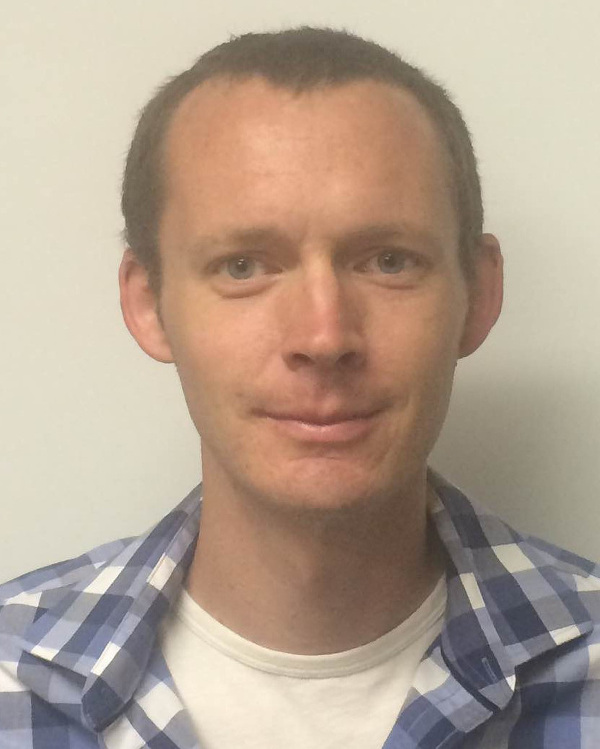
\includegraphics[width=1 in,height=1.25in,clip,keepaspectratio]{figures/braker_headshot.jpg}}]
  {Roger A. Braker} earned the B.A. degree in physics from the University of Oklahoma in 2005 and the M.S. degree in electrical engineering from the University of Colorado in 2017.
  Since 2014, he has been a graduate student in the Electrical, Computer, and Energy Engineering
  Department at the University of Colorado Boulder.

\end{IEEEbiography}

\begin{IEEEbiography}
  [{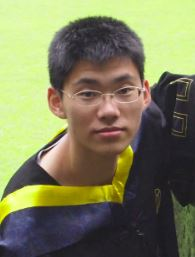
\includegraphics[width=1 in,height=1.25in,clip,keepaspectratio]{figures/yufan.JPG}}]
  {Yufan Luo}
received dual B.S. degrees in automation and in management science from Zhejiang University, Zhejiang, China, in 2011, an M.S. degree in industrial and operations engineering from the University of Michigan, Ann Arbor, MI, USA, in 2012, and a Ph.D. degree in systems engineering from Boston University in 2019. He is currently with Juniper Networks, Sunnyvale, CA.

\end{IEEEbiography}

\begin{IEEEbiography}
  [{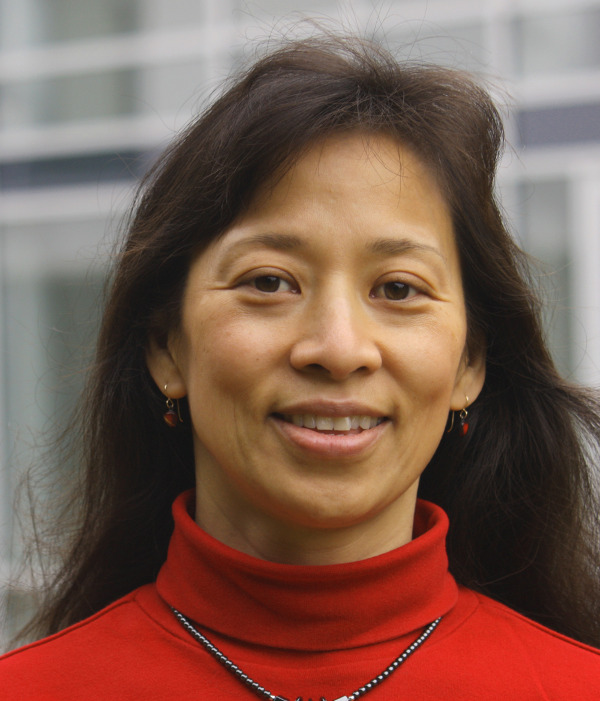
\includegraphics[width=1 in,height=1.25in,clip,keepaspectratio]{figures/pao_headshot.jpg}}]
  {Lucy Y. Pao} 
  is the Palmer Endowed Chair Professor in the Electrical, Computer, and Energy Engineering Department at the University of Colorado Boulder. She earned B.S., M.S., and Ph.D. degrees in Electrical Engineering from Stanford University. Her research has primarily focused on engineering control systems, with applications ranging from atomic force microscopes to multi-megawatt wind energy systems. She is a Fellow of the IEEE and the International Federation of Automatic Control (IFAC). Selected recent awards include the 2012 IEEE Control Systems Magazine Outstanding Paper Award, the 2015 Society for Industrial and Applied Mathematics (SIAM) Journal on Control and Optimization Best Paper Prize, the 2017 Control Engineering Practice Award from the American Automatic Control Council, and the Scientific Award 2017 from the European Academy of Wind Energy. Selected recent and current professional society activities include being a Fellow of the Renewable and Sustainable Energy Institute (2009-present), 
  General Chair of the 2013 American Control Conference, member of the IEEE Control Systems Society (CSS) Board of Governors (2011-2013 and 2015), IEEE CSS Fellow Nominations Chair (2016-2018), and member of the IFAC Executive Board (2017-2020).    

\end{IEEEbiography}

\begin{IEEEbiography}
  [{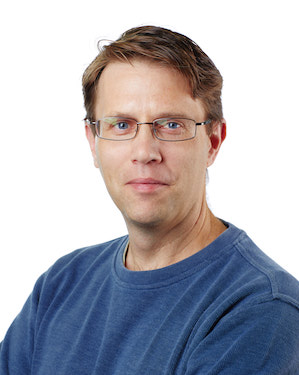
\includegraphics[width=1 in,height=1.25in,clip,keepaspectratio]{figures/SeanAndersson_IEEE.jpg}}]
  {Sean B. Andersson}
received the B.S. degree in engineering and applied physics from Cornell University, Ithaca, NY, USA, in 1994, the M.S. degree in mechanical engineering from Stanford University, Stanford, CA, USA, in 1995, and the Ph.D. degree in electrical and computer engineering from the University of Maryland, College Park, MD, USA, in 2003. He has worked at AlliedSignal Aerospace and Aerovironment, Inc. and is currently an Associate Professor of mechanical engineering and of systems engineering with Boston University, Boston, MA, USA. His research interests include systems and control theory with applications in scanning probe microscopy, dynamics in molecular systems, and robotics. He received an NSF CAREER award in 2009, is a senior member of the IEEE, and was an associate editor for the IEEE Transactions on Automatic Control (2014-2018) and for the SIAM Journal on Control and Optimization (2013-2018).
\end{IEEEbiography} 

%%%%%%%%% then the Bibliography, if any %%%%%%%%%
% \bibliographystyle{plain} % or "siam", or "alpha", etc.
\bibliographystyle{IEEEtran} % or "siam", or "alpha", etc.
% \nocite{*} % list all refs in database, cited or not
\bibliography{braker_bibs,Andersson_bibs,Yufans_bibs} % Bib database in "refs.bib"


%%%%%%%%% then the Appendices, if any %%%%%%%%%
\end{document}

